\chapter{Approach}
\label{chapter:approach}

In the following passage, the hardware and software construction used
in this work will be discussed.  Specifically, details of the parallelization and
reduction strategies, will be elaborated.  The full source code can be found in
appendix \ref{appendix}, but excerpts will be inserted into the following passages
where suitable.

\section{Experiment Hardware}
For the numerical experiments conducted during this research, two hardware configurations
are used.  First, a dual GPU configuration consisting of two NVIDIA GTX 560Ti GPU's is
employed to test multi-device capabilities. Also, seeing as these devices
could only run \Gls{CUDA} code complied for compute architecture 2.1, code
backwards compatibility was also tested with this set up.
The second compute configuration consists of an NVIDIA TITAN X GPU, which allowed
the testing of the compute architecture 6.1.
\par
Both \Gls{GPU} configurations were run used with the same Fujitsu D3067-A1 mother board,
with 16GB or RAM and an Intel Xeon CPU, model E31235 running at 3.20GHz.

\section{Parallelization}
In order to successfully map a mathematical problem to specific hardware, one must
consider the three main bottle necks of parallel computing, namely,
memory allocation and access strategies, execution order and data communication.
The complete implementation, can be found and referenced in appendix \ref{appendix}.
In the following passages, some of the intricacies of the implementation will be
elaborated.

\subsection{Thread-level Parallelism}\label{tlp}
Commonly, one wishes to store heavily used data in shared memory in oder to
take advantage of the increased data access speeds and inter-block data sharing
capabilities.  For this reason, the \textit{direction}, \textit{radius}, and \textit{position}
vectors were all stored allocated in shared memory, contributing a shared memory usage of
$3N$.
\begin{lstlisting}[caption="src/wos\_native.cuh",label=BlockVariablePointers]

  struct BlockVariablePointers {
    float *s_radius, *s_direction, *s_cache, *s_x, *s_result;
  };
  __device__ void calcSubPointers(BlockVariablePointers *bvp, size_t len,
                                  float *buff) {
    bvp->s_radius = buff;
    bvp->s_direction = len + buff;
    bvp->s_cache = 2 * len + buff;
    bvp->s_x = 3 * len + buff;
    bvp->s_result = 4 * len + buff;
  }
  __device__ void smemInit(BlockVariablePointers bvp, float *d_x0, int tid) {
    // initialize shared memory
    bvp.s_direction[tid] = 0.0;
    bvp.s_cache[tid] = 0.0;
    bvp.s_radius[tid] = INFINITY;
    // copy x0 to local __shared__"moveable" x
    bvp.s_x[tid] = d_x0[tid];
    if (threadIdx.x == 0)
      bvp.s_result[0] = 0.0;
  }
\end{lstlisting}

For each dimensional vector entry, one thread was assigned, subsequently
also leading to a \textit{blocksize} of $N$.  The practice of one tread per vector
entry is a common pattern in many \Gls{GPGPU} as is the pattern of storing data in shared
memory and using one thread per data entry enables efficient data communication
between threads and accelerated data reads from shared memory. In order to allocate,
and initialize and manage multiple variables in shared memory, a pointer structure and helper functions
were used.  This structure was initialized locally per thread and pointed to an
external allocation of shared memory $buff[ ]$.

Each of the steps of \Gls{RWoS} was implemented thread-wise.  A thread-wise implementation
explicitly defines a each step as a kernel for individual vector entries.  Each of these operations
can be executed in parallel by its respective thread.  Where communication is necessary,
shared memory access and a function call $\_\_syncthreads()$ in order to avoid \Gls{rc}.

\subsection{Block-level Parallelism}
Due to the lack of communication necessary between independent paths and their
their subsequent boundary evaluations, the mapping to \Gls{CUDA} blocks lends itself
to the  application.  For the evaluation of $P$ \Gls{RWoS} paths, $P$ CUDA blocks
of dimension $N$ are allocated.  Each local Path evaluation result is saved in the $s\_result$
variable in the shared memory structure \ref{BlockVariablePointers}.
\par
In mapping every path to a specific block, one limits oneself to the bounds of the
CUDA hardware.  Currently, the greatest number of blocks available for execution
of one kernel limited to the value $MAX\_BLOCKS = 65535$.  In oder to reach a greater
iteration count, a strategy was devised to split a number of total paths greater
than $MAX\_BLOCKS$ linearly on to a smaller number of \Gls{CUDA} resources.  In short,
for every path evaluation $P$ greater than $65535$, each block will conduct $floor(P/65535)$
path iterations. The remaining path iterations, $R = P \% 65535$ will be conducted
 by the first $R$ blocks of the grid.  This strategy,
although primitive, was found through testing to yield the greatest performance,
compared to all other tested strategies. One can assume, this is due to greater
explicit dependency independence that the a block exhibits.  All other alternatives,
involved a greater number of "sequential" path evaluations per block, and therefore
a greater overall running time.   Meanwhile, by maximizing the number of blocks,
one creates greater parallelism in the program that can be exploited on a \Gls{GPGPU}.
An excerpt of the implementation can be found below.

\begin{lstlisting}[caption="src/gpu\_config.cpp Appendix \ref{appendix}",label=block-parallelism-strategy]
  ...
  // uppdate paths per block
  if (gpuPaths <= MAX_BLOCKS) {
    numberBlocks = gpuPaths;
    blockIterations = 1;
    blockRemainder = numberBlocks;
  } else {
    numberBlocks = MAX_BLOCKS;
    blockIterations = ceil((gpuPaths / (float)MAX_BLOCKS));
    blockRemainder = gpuPaths % MAX_BLOCKS;
  }
...
\end{lstlisting}

\subsection{Device-level Parallelism} \label{devicePar}
In order to decrease running time, it is advantageous to map the problem at hand
to multiple devices.  In the course of this work, this was realized through a
simple stream based distribution to two devices connected by a common PCIe bus.
The strategy for device level parallelism was precedes the block-level parallelism
strategy, and merely divides the total number of paths desired, by the number of
available devices.
\begin{lstlisting}[caption="src/gpu\_config.cpp Appendix \ref{appendix}",label=device-parallelism-strategy1]
  //...
// nGPU
checkCudaErrors(cudaGetDeviceCount(&nGPU));
gpuPaths = p.totalPaths / nGPU;
  //...
\end{lstlisting}

\begin{lstlisting}[caption="src/wos\_native.cuh Appendix \ref{appendix}",label=device-parallelism-strategy2]
  for (int i = 0; i < gpu.nGPU; i++) {
    checkCudaErrors(cudaSetDevice(i));
    checkCudaErrors(cudaStreamCreate(&multiGPU[i].stream));
    //...
    }
  //...
  for (int i = 0; i < gpu.nGPU; i++) {
    checkCudaErrors(cudaSetDevice(i));

    dim3 dimBlock(gpu.numThreads, 1, 1);
    dim3 dimGrid(gpu.numberBlocks, 1, 1);

    cudaError err;

    WoS<<<dimGrid, dimBlock, gpu.size_SharedMemory, multiGPU[i].stream>>>(
        multiGPU[i].d_x0, multiGPU[i].d_paths, multiGPU[i].d_avgPath,
        multiGPU[i].d_stepCount, p.eps, p.x0.dimension, p.avgPath,
        gpu.blockIterations, gpu.blockRemainder, i + 1);
    err = cudaGetLastError();
    if (cudaSuccess != err) {
      printf("Wos Kernel returned an error on device %d:\n %s\n", i,
             cudaGetErrorString(err));
    }
  }
  //...
\end{lstlisting}



\subsection{Reduction}
Data reduction describes the act of consolidating a large amount of values to
a individual value or subset of values by means of a numerical or logical operations.
Although summation is a common example, other reduce operations include,
but are not limited to maximum value, minimum value, product and bitwise reduce operations.
  Commonly,
sum-reduce describes the addition of all data values in a set and returning a single value.
In sequential execution, a reduce operation will, for $N$ input values, have a nominal
running time of $0(N)$ and is most commonly realized by means of a loop over that
input data.  In parallel computing, these operations are performed in parallel by dividing the,
workload among the $w$ worker cores and performing serial reduction of the subsets,
while finally reducing the intermediate results.  This naive approach leads to an
optimal \gls{speed-up} of $w$.  Due to the lack of a global synchronization mechanism
on \Glspl{GPU}, this naive reduction parallelization approach is not possible,
and other methods have been developed.  Mark Harris, dives deep into the benefits
and pitfalls of parallel reduction on \Glspl{GPU} and has derived optimized
recursive approaches, as documented in \cite{harris}.  Some key points from his work are
the avoidance of:
\begin{description}
  \item [Avoidance of branch divergence]
since each warp executes one common instruction at a time, when branch divergence,
(i.e. if/else evaluation) occurs for individual elements, the warp-wise execution pattern
is broken, and additional warps must be executed for diverging threads. This \Gls{GPU} anti-pattern
leads to execution overhead and a subsequent loss in performance
  \item [Bank conflict free addressing strategies]
  in order to achieve the improved performance and concurrent read and write capabilities
  of shared memory, memory is divided into equally sized sub modules, called banks.
  These sub modules can be accessed by independent threads in parallel, allowing a speed up
  of $B$ for $B$ separate memory banks.  When multiple threads request access to
  the same memory bank, the accesses are serialized, therefore restricting the performance increase.
  These access patterns are called bank conflicts, and can drastically decrease
  the performance of shared memory.  To avoid bank conflicts, a coalesced data
  access pattern is recommended.
  \item [Loop unrolling] by explicitly defining looped operations, the loop overhead
  can be reduced to a minimum, therefore allowing for greater performance during execution.
  \item [compile time evaluation]  In order to reduce the number of conditional
  evaluated at runtime, the C++ feature of templating can allow compile-time statement
  evaluation, for example concerning block and thread dimensional conditional statements.
  This pattern further increases code performance on \Glspl{GPU}
\end{description}

  \begin{lstlisting}[caption="src/wos\_native.cuh",label=sumReduce]
    //...
    __device__ void warpSumReduce(float *sdata, int tid) {
      // each thread puts its local sum value into warp variable
      float mySum = sdata[tid];
      unsigned int blockSize = blockDim.x;

      // do reduction in shared mem

      if ((blockSize == 1024) && (tid < 512)) {
        sdata[tid] = mySum = mySum + sdata[tid + 512];
      }

      __syncthreads();

      if ((blockSize >= 512) && (tid < 256)) {
        sdata[tid] = mySum = mySum + sdata[tid + 256];
      }

      __syncthreads();

      if ((blockSize >= 256) && (tid < 128)) {
        sdata[tid] = mySum = mySum + sdata[tid + 128];
      }

      __syncthreads();

      if ((blockSize >= 128) && (tid < 64)) {
        sdata[tid] = mySum = mySum + sdata[tid + 64];
      }

      __syncthreads();

    #if (__CUDA_ARCH__ >= 300)
      if (tid < 32) {
        // Fetch final intermediate sum from 2nd warp
        if (blockSize >= 64)
          mySum += sdata[tid + 32];
        // Reduce final warp using shuffle
        for (int offset = warpSize / 2; offset > 0; offset /= 2) {
          mySum += __shfl_down(mySum, offset);
        }
      }
    #else
      // fully unroll reduction within a single warp
      if ((blockSize >= 64) && (tid < 32)) {
        sdata[tid] = mySum = mySum + sdata[tid + 32];
      }

      __syncthreads();

      if ((blockSize >= 32) && (tid < 16)) {
        sdata[tid] = mySum = mySum + sdata[tid + 16];
      }

      __syncthreads();

      if ((blockSize >= 16) && (tid < 8)) {
        sdata[tid] = mySum = mySum + sdata[tid + 8];
      }

      __syncthreads();

      if ((blockSize >= 8) && (tid < 4)) {
        sdata[tid] = mySum = mySum + sdata[tid + 4];
      }

      __syncthreads();

      if ((blockSize >= 4) && (tid < 2)) {
        sdata[tid] = mySum = mySum + sdata[tid + 2];
      }

      __syncthreads();

      if ((blockSize >= 2) && (tid < 1)) {
        sdata[tid] = mySum = mySum + sdata[tid + 1];
      }

      __syncthreads();
    #endif

      if (tid == 0)
        sdata[0] = mySum;

      __syncthreads();
    }
    //...
\end{lstlisting}
Briefly, the $\_\_\_shfl\_down(...)$ command should be examined. Before, compute capability
3.0 (Kepler), reductions between warps of the same thread had to be completed in
shared memory.  This meant that data transfers between warp registers and shared
memory had to be completed for every reduction step.  Since Kepler, warps have gained
the capability to directly access values stored in neighboring warps registers,
thereby increasing effective bandwidth, freeing shared memory and eliminating the
necessity for warp synchronization. This action was cleverly named shuffle \cite{shuffle}.
\subsubsection{Local Reduction}\label{localRed}
Based on \cite{harris}, optimized reduction kernels were introduced for efficient
shared memory minimum and summation reductions needed for \Gls{RWoS}\ref{appendix}.
In order to successfully use these optimized reduction techniques, the memory allocations
discussed in \ref{tlp} were step-wise over allocated, meaning it was ensured that
the total size of allocated shared memory could store a power of 2 number of elements,
regardless of the required dimension.  Unused elements were initialized with with
values which would remain constant during the entire simulation (e.g. 0 and INFINITY).
This strategy allowed for coalesced warp-wise memory accesses, that minimized
thread divergence and despited the computational overhead, lead to performance gains
of $~50\%$ compared to initial naive reduction implementations.
\subsubsection{Global Reduction}
The global reduction of path evaluation results is realized through a serial
a $cudaMemcpyAsync(...)$ to the host, and a serial host reduction.  This strategy
proved to provide greater performance than a restructuring of the CUDA thread/Block
allocation and subsequent GPU reduction, due to the minimization of GPU configuration
overhead.  In order to reduce the numerical error of floating point reduction,
Kahan's summation algorithm was employed.
\begin{lstlisting}
  float reduceCPU(float *data, int size) {
    float sum = data[0];
    float c = 0.f; // numerical summation error variable

    for (int i = 1; i < size; i++) {
      float y = data[i] - c; // subtract previous error
      float t = sum + y; // add corrected value to intermediate sum
      c = (t - sum) - y; // recalculate error
      sum = t; // set new intermediate sum
    }
    return sum;
  }
\end{lstlisting}

\section{Random Number Generation}
In order to generate pseudo random numbers for the random directions necessary
for \Gls{RWoS}, the \Gls{CUDA} library \Gls{CURAND} was utilized.
\subsection{CURAND}
The \Gls{CURAND} library provides an API necessary for generating high quality
pseudo random numbers.  The default pseudo random number generator XORWOW was
was used during this work\cite{xorwow}.  The CURAND implementation of XORWOW provides
a seed dependent, reproducible series of random numbers, that has
a period greater than $2^{190}$. By modulating the seed, the user is guaranteed a
different starting state and subsequent different series of pseudo-random numbers.
The device API of \Gls{CURAND} allowed
the generation of pseudo random numbers during the execution of \Gls{RWoS} and
therefore greatly reduce the amount of data transfer to the device, and therefore
the overall running time of the program.  Furthermore, the pseudo-random normal
distribution functionality of \Gls{CURAND} was used to generate normal distributions
in an $N$-dimensional euclidean space, which subsequently created a uniform spherical
distribution.
%\subsection{Pseudo-Random and Quasi-Random}
\subsubsection{Seed Independence}
In order to generate independent pseudo-random directions in every dimension,
a thread independent seed was selected, seen below.
\begin{lstlisting}[caption="Random Number Generation(source:src/wos\_native.cuh see: appendix \ref{appendix})",
  label=Random Number Generation]
  int index = threadIdx.x + blockDim.x * blockIdx.x;
  int tid = threadIdx.x;

  curandState s;
  // seed for random number generation
  unsigned int seed = index * gpu;
  curand\_init(seed, 0, 0, &s);
\end{lstlisting}
By using the global thread index as a seed, one can strive to achieve independent
sequences of pseudo-random numbers in every direction, for every path.  In order,
to guarantee the randomness caries over when using a multi-GPU hardware configuration,
the GPU-ID (starting from 1) is multiplied with the the thread index seed in order
to ensure seed independence throughout the simulation.

\subsection{Excursion: uniform random directions on a Sphere}\label{uniformPoints}

In the process of understanding how the generation of uniform distributions on
spherical surfaces can be created, the following 2 dimensional practical exemplary
experiments were performed.

In order to attain a distribution on a sphere, the process followed in this work,
consisted of creating an $N$-dimensional normal distribution in euclidian space and
sampling from the afore mentioned distribution.  The $N$-dimensional sample vector
is subsequently normalized onto the $N$-dimensional unit sphere.  Below, the process
exemplarily visualized for a 2D example.  Furthermore, the 2D case of a uniform
euclidian distribution being normalized is also exemplified, in order to intuitively
show the distributional discrepancies and obvious ill suited nature for the problem
at hand.  The two point clouds below are 2D normal and uniform distributions
respectively.  The peaks on the uniform distribution histogram stem from the corners
of the distribution in a 2 dimensional euclidian distribution.  When projected onto
the sphere, the accumulation of points in the corner of the euclidian domain create
''hot spots'' in the spherical distribution.  The two dimensional normal
distribution point cloud on the other hand, mitigates this problem due to the summation
of the tails of the distributions in the 1D plane, leading to a low probability
in the corners of the square domain.  When the point cloud  is subsequently projected
onto the sphere, it lacks the peaks in the  spherical distribution and displays an
overall uniform nature as can be seen in the relatively constant levels  histogram below.
\begin{figure}
\begin{center}
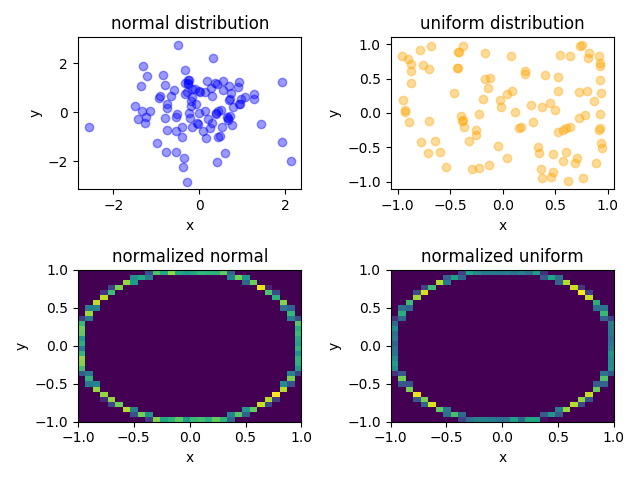
\includegraphics[width=10.0cm]{styles/distributions} \label{plot:distributions}
  \caption{}
  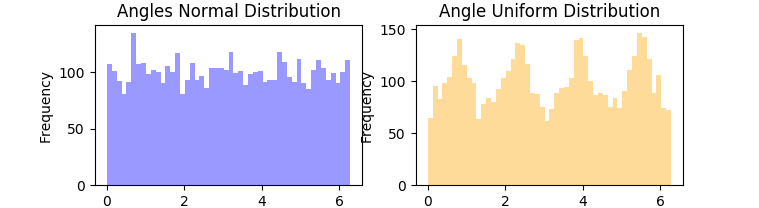
\includegraphics[width=10.0cm]{styles/histograms} \label{plot:historam}
    \caption{}
\end{center}
\end{figure}


%The connection between normal distributions and spheres is not merely

%http://math.stackexchange.com/questions/28558/what-do-pi-and-e-stand-for-in-the-normal-distribution-formula
